
\section{Experiments}
\label{sec:expts}

\subsection{Parameters}
\label{subsec:enum}
Some of the key parameters that we had to decide on for our genetic program were generation size, number of generations, and the percentage of individuals to perform each of our genetic operations on. For generation size, we stuck with 50 individuals because of the diversity and speed that it provided. In general, lower generation sizes yielded less diversity leading to lower plateaus of the best team's score while significantly higher generation sizes lead to significantly slower run time. For number of generations, we played around with this depending on what we were testing, however, 250 generations seems to give a good idea of what the final team will look like. This number might change depending on some of the variations of the genetic operations we implement. We will discuss the effects of number of generations later in this section. Concerning genetic operations, the breakdown of DraftKing's percentages are the following: crossover on $80\%$ of individuals, mutation on $15\%$ of individuals, and regeneration of $5\%$ of individuals. We decided on these percentages because they gave DraftKing the ability to make significant improvements with crossovers, yet mutate a decent number of individuals in attempt to fine-tune the lineups. Mutation was especially important given that crossover indices were selected to make sure groups of players in the same position were not broken up to avoid duplicate players. Therefore, if the first starting pitcher was selected as the crossover point, all the starting pitchers would be crossed over. Mutation would then allow this group of starting pitchers to be modified. Regenerating $5\%$ of individuals made sure that some of the most fit individuals will be carried onto the next generation, keeping their quality traits in the gene pool. 


\subsection{Implementing Selective Mutation}
\label{subsec:enum}
During initial experimentation, we used basic crossover, mutation, and reproduction as described in the Background section. We were able to get solid lineups, however, it took hundreds of generations to reach them. We decided to create a selective mutation operation that mutated weak parts of a team. Initially, we created a selective mutation method that chose a mutation index based off the player with the worst value on the team determined by the equation $points_x \div points_{team} - cost_x \div cost_{team}$ where $x$ is the current player and $team$ is the entire team. Once this player was selected, they were randomly replaced with another player. However, we realized that this player was often replaced with a player with fewer points. Even though they were a better value based on our equation, they did not help maximize the team's score. This method of mutation did not account for the fact that we had a budget that could be used fully without consequence. This method would be much more useful to maximize a lineup at minimum cost. Therefore we implemented a cutoff at $90\%$ of the total budget. Any team with less than this cutoff value would be mutated using a different metric. This metric was a player's points. The mutation index for all teams with a cost less that this cutoff value would be that of the player with the least amount of points. The combination of these two metrics was extremely effective. The program now was able to realize that it could splurge on expensive players when the budget was there, significantly increasing the point total. We were also then able to find more optimal lineups when the budget got tight, replacing overvalued players with more successful cost-efficient players. We will now compare this mutation method to regular random mutation.


\subsection{Regular Mutation vs. Selective Mutation}
\label{subsec:enum}
Our main experiment consisted of testing regular random mutation vs. selective mutation, seeing how total points varied between genetic programs using the two methods after a certain amount of generations. All runs were completed with a generation size of 50 individuals and crossover, mutation, and reproduction ratios of $0.8$, $0.15$, and $0.05$. The results are seen in Figure 1.



\begin{figure}
\centering
    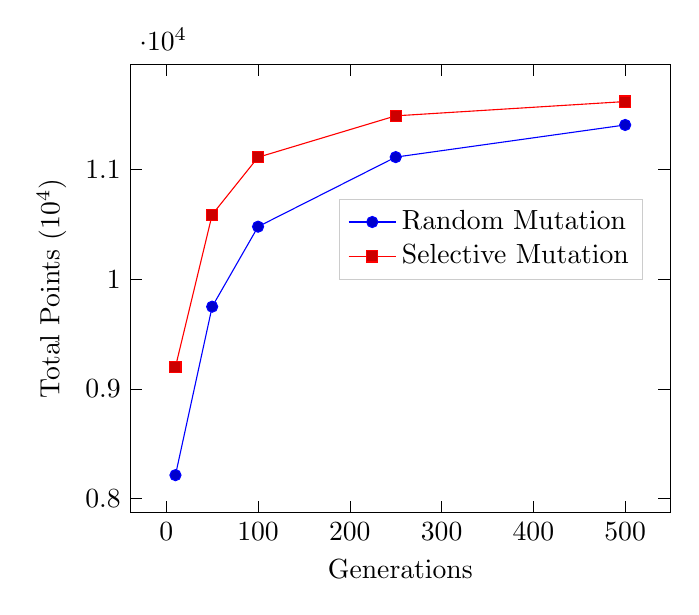
\begin{tikzpicture}
      \begin{axis}[
        legend cell align={left},
        legend style={draw=white!80.0!black, at={(.95,.7)},anchor= north east},
        x grid style={white!69.01960784313725!black},
        xlabel={Generations},
        xtick style={color=black},
        y grid style={white!69.01960784313725!black},
        ylabel={Total Points ($10^4$)},
        ytick style={color=black}
        ]
        \addplot coordinates {
          (10,  8214.6)
          (50,  9751.2)
          (100,  10481.0)
          (250, 11115.5)
          (500, 11408.6)
        };
        \addlegendentry{Random Mutation}
        \addplot coordinates {
          (10,  9201.5)
          (50,  10590.8)
          (100,  11113.9)
          (250, 11491.9)
          (500, 11622.1)
        };
        \addlegendentry{Selective Mutation}
      \end{axis}
    \end{tikzpicture}
\caption{Plot showing the progression of average total team scores of genetic programs with selective mutation versus those with random mutation. Each point represents the average team points total for 10 runs at a given generation size.}
\end{figure}





Based on this experiment, it is clear that the selective mutation is more effective at building better teams quicker. This makes sense given that when selective mutation is used, a team's weakness is most definitely improved upon mutation, while random mutation could easily make the player at a given position worse. This experiment also gives us an idea of the number of generations needed to find the optimal team. Based off the averages and Figure 1, it is clear that teams are still improving up until 500 generations in both cases. We believe that after 500 generations, a team is very near, if not at, the peak of where it can get. Especially when using selective mutation, we saw little to no improvement once generations got near 500, as seen in the plateauing of selective mutation in Figure 1. Runs using regular mutation might still see a bit of improvement after 500 given that these teams tend to plateau after higher numbers of generations. Overall, Figure 1 demonstrates that selective mutation significantly increases the effectiveness and speed of our genetic program.
